\chapter{\label{sec:dispmapcreation} Displacement Maps}

The layered animation method presented above allows animation of complex datasets, but requires recalculation of every detail layer vertex in each frame in order to render the final surface. While this gives the maximum level of realism and accuracy possible with the layered animation model, it requires too much computation to use for anything other than non-realtime, offline rendering. In this model, only the low-resolution control layer is suitable for real-time rendering. 

Ideally, we would like to be able to regenerate the detailed surface at an arbitrary level of detail, allowing us to control the trade-off between the amount of surface detail and the calculation time required. This would allow us to render the model at any level of detail we like, from a basic model for realtime manipulation, to a full-detail surface for offline rendering. This would allow our representation to be used in many more application areas, from games to film production.

Therefore, we require an alternative representation of the detail layer, which will enable us to choose how much of the surface detail is reconstructed, and in which areas of the model. We can then produce animated reconstructions that are more detailed than the control layer, but can still be rendered in real time. Such a representation may also allow us to edit the detailed surface in a simple manner, and also to compress the detailed surface data into a more compact form.

We require a number of properties for our alternative parameterisation. The most important property is that if we are to work with arbitrary levels of detail, we must be able to obtain the correct value of the detail layer for any point on the control layer, not just those corresponding to detail layer vertices. The parameterisation should also preserve as much detail as possible from the original surface, and animate in the same smooth manner as the detail layer in our original layered animation approach.

We therefore choose to represent the detail layer as a {\it displacement map} defined over the control layer. The displacement map is an error function whose value represents the difference between two surfaces. This error function can be either a vector or scalar field, depending on the required properties. As we only need to encode a single value, i.e. the distance along the surface normal for each point on the control layer, we only require a scalar displacement field. Choosing a scalar-valued field also has advantages in that the representation is more compact, requiring only one parameter per sample point, as opposed to three for a vector field.

If we {\it unwrap} the three-dimensional control layer onto a two-dimensional plane, we can assign the displacement values for the detail layer to points on this 2D plane. The displacement field is sampled at each point on the plane, so that as well as storing displacements for each of the vertices in the original detail layer, we also store values for all points on the control layer mesh in between these vertices. Once the detail layer is encoded in this form, we have much more flexibility in reconstructing the surface detail, as we can choose to recreate an arbitrary part of the surface, including parts that did not exist as vertices in the original detail layer. 

As the error function is scalar, and each point on the 2D plane has only a single value, we can store the displacement map as an image which is mapped to the 3D surface. However, instead of encoding surface colour, the displacement image encodes the scalar error value between our low and high resolution surfaces for each pixel. 

\section{\label{sec:dispmapcreation:overview}Algorithm Overview}

The process of generating a displacement map consists of a number of stages. First, we define a valid mapping from the surface of the 3D control mesh to a 2D image plane. Then, we generate the displacement map by storing the error between the control and detail layers at each point as the value of a pixel on the image plane.

\begin{figure}
\begin{center}
\setlength{\unitlength}{0.4cm}
\begin{picture}(18,12)
% Control Mesh
\thicklines
\put(0,6){\circle*{0.2}}
\put(0,6){\line(1,1){6}}
\put(0,6){\line(2,-1){12}}
\put(6,12){\circle*{0.2}}
\put(6,12){\line(1,-2){6}}
\put(6,12){\line(3,-1){12}}
\put(12,0){\circle*{0.2}}
\put(12,0){\line(3,4){6}}
\put(18,8){\circle*{0.2}}
% T^E
\thinlines
\put(7,5){\line(3,1){3}}
\put(7,5){\line(2,3){2}}
\put(10,6){\line(-1,2){1}}
% T^I
\put(11,8){\line(2,-3){2}}
\put(11,8){\line(3,-1){3}}
\put(13,5){\line(1,2){1}}
\end{picture}
\caption[Internal and External Triangles]{\label{fig:intexttriangles} Internal and External Triangles. The large triangles represent the control mesh. The small detail layer triangle on the left is a member of ${\cal T}^E$, while the one on the right is a member of ${\cal T}^I$.}
\end{center}
\end{figure}

We must calculate displacement values for each pixel in the displacement map. We do this by drawing each detail layer triangle $t \in {\cal T}$ into the displacement map in turn. We can treat each triangle individually, and calculate the displacement map for one detail triangle at a time. For reasons explained below, we must use two separate methods for doing this, depending on whether the detail triangle is contained wholly within one control layer triangle or not.

We therefore divide the set of detail layer triangles ${\cal T}\symbol{triset}$  into two mutually exclusive sets, ${\cal T}^I$ and ${\cal T}^E$. ${\cal T}^I$ represents the set of {\it internal} triangles, which are wholly contained within the normal volume associated with a single control layer triangle, i.e. all their vertices are mapped to the same control triangle as described in section \ref{sec:scandata:creation:mapping}. Conversely, ${\cal T}^E$ represents the set of {\it edge} triangles, which do not fulfil this criterion, and whose vertices map to more than one control layer triangle. This distinction is illustrated in figure \ref{fig:intexttriangles}.

The general process of displacement map creation is summarised in algorithm \ref{alg:dispmapping}, and is explained in detail in the following sections.

\begin{algorithm}[tbp]
\begin{algorithmic}
\IF{Control layer does not have pre-existing texture coordinates.}
	\STATE Generate texture coordinates for control layer
\ENDIF
\FORALL {$t \in {\cal T}$}
	\IF {$t \in {\cal T}^I$}
		\STATE Resample $t$ into the displacement map
	\ELSE
		\FORALL {normal volumes $N \in {\cal N}$ that contain part of $t$}
			\STATE Calculate the geometric intersection ${\cal I} = t \cap N$
			\STATE Resample ${\cal I}$ into the displacement map
		\ENDFOR
	\ENDIF
\ENDFOR
\end{algorithmic}
\caption{\label{alg:dispmapping}Displacement Map Generation}
\end{algorithm}

\section{\label{sec:dispmapcreation:unwrap}Texturing the Control Layer}

In order to generate a displacement map for our high-resolution detail layer, we must first define a bijective mapping from the 3D control layer to a 2D image representation, by defining {\it texture coordinates} for the mesh\footnote{This mapping is one-to-one when each control triangle is considered individually, but not for the mesh as a whole. For instance, an edge in the control mesh may have two locations in the image plane, and a vertex may have any number. The values for all instances of an edge or vertex in the image plane should be the same, however, so this is not a problem.} . If we do not already have manually-defined texture coordinates for the control layer mesh, we must automatically generate this information. We must map each triangle in the control layer to a separate area in the image, into which we will store the displacement values for that triangle.

There are a number of properties we would like in our mapping into the 2D texture domain. Ideally, triangle adjacency should be preserved as much as possible; i.e. triangle which share edges in the mesh should also share them in the image domain. This property makes it easy for the resulting images to be edited as a whole; it would be much harder to edit a displacement map composed of multiple disjointed triangles. We would also like to preserve the relative sizes of the triangles, so that a large triangle is sampled more densely than a small one, allowing us to subdivide it further with a high level of accuracy.

The simplest option for generating texture coordinates is to simply ignore the geometric information in the control mesh, and assign texture coordinates to each triangle in a regular pattern. An example of such as pattern is shown in figure \ref{fig:texcoords}a. As each triangle is considered individually, this method ignores both triangle adjacency and relative size. However, it does guarantee a bijective mapping.

An alternative to the regular mapping above is a {\it cylindrical} mapping \cite{Lengyel02}, shown in figure \ref{fig:texcoords}b. For this method, each mesh vertex is converted into a cylindrical coordinate system whose origin is the centroid of the mesh. The cylindrical coordinate system represents a point $\vec{p}$ as a combination of the parameters $r$, $\phi$ and $y$. $r$ is the straight-line distance from the origin to $\vec{p}$, $||\vec{p}||$. The {\it azimuth} value, $\phi$, is the angle between the plane $x=0$ and $\vec{p}$. The $y$ value has the same meaning as in a standard Cartesian coordinate system, and represents the height above the plane $y=0$. Once these coordinates have been calculated for each point, normalised $\phi$ and $y$ values are used to define 2d coordinates on the image plane. The $r$ coordinate is ignored.

Closely related to the cylindrical method described above is {\it spherical} mapping \cite{Lengyel02}. This is identical to the cylindrical case, except that the $y$ coordinate is replaced by $\theta$, the {\it polar angle}. This represents the angle between the vector $\vec{p}$ and the plane $y=0$. The $\phi$ and $\theta$ coordinates are normalised to the range 0 to 1 and used as a 2D coordinate in the image plane. Spherical mapping is shown in figure \ref{fig:texcoords}c.

While the two methods above preserve some adjacency and size information, they do not guarantee a bijective mapping, as it is possible for triangles to overlap when mapped to the enclosing cylinder or sphere. We can generate a map that give us the best features of the previous three methods by using the {\it pelting} method, proposed by \citet{Piponi00}, which is illustrated in figure \ref{fig:texcoords}d. In this method, a set of mesh edges are defined as seams, along which the mesh will be split. These seams are then ``stretched'' out, until the mesh is flattened, at which point texture coordinates can be simply inferred from the coordinates of the vertices. However, one drawback of this method is that relative sizes of triangles in the original mesh are very difficult to preserve or control in any predictable way.

\begin{figure}
\begin{center}
\begin{tabular}{cccc}
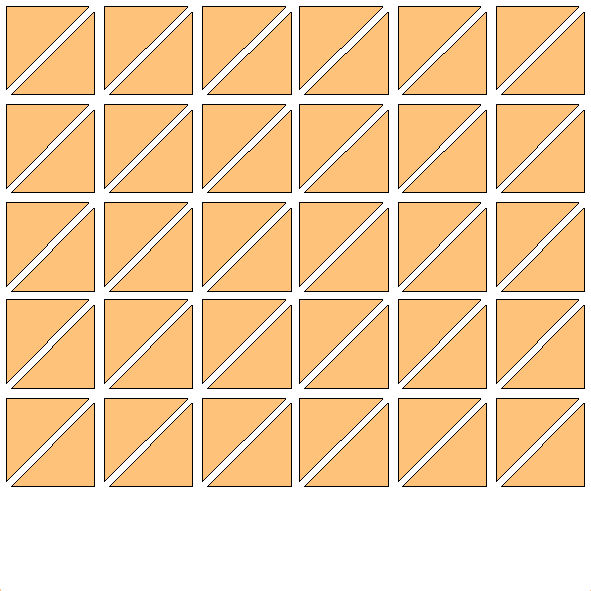
\includegraphics[width=3.2cm]{../images/texcoord_reg} &
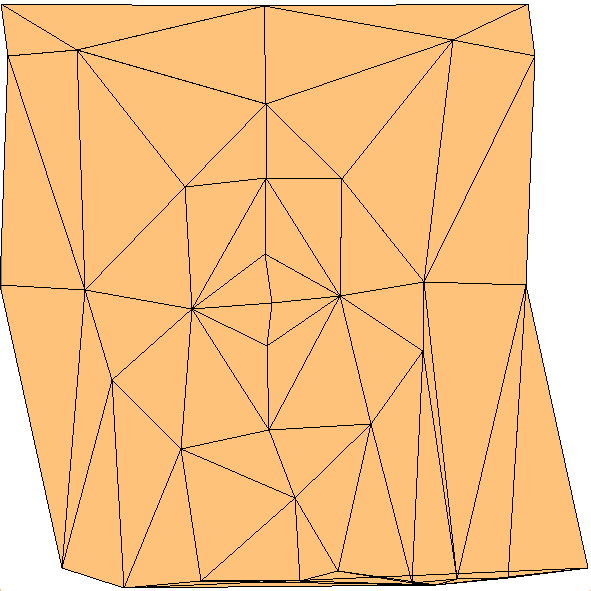
\includegraphics[width=3.2cm]{../images/texcoord_cyl} &
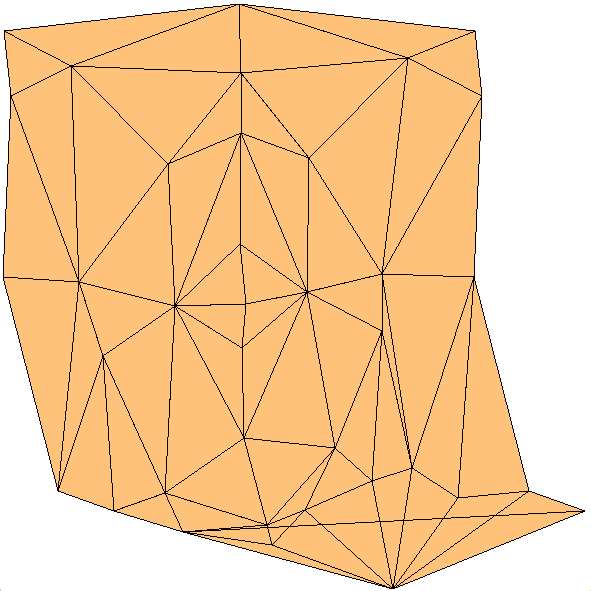
\includegraphics[width=3.2cm]{../images/texcoord_sph} &
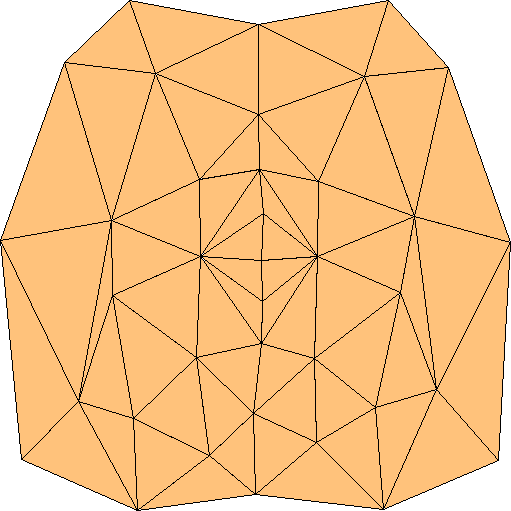
\includegraphics[width=3.2cm]{../images/texcoord_plt} \\
{\it (a)} & {\it (b)} & {\it (c)} & {\it (d)}
\end{tabular}
\caption[Texturing Methods]{\label{fig:texcoords} Texturing Methods, generated for the Monster head control model. (a) Regular. (b) Cylindrical mapping. (c) Spherical mapping. (d) Pelting.}
\end{center}
\end{figure}

In this research, where pre-existing texture coordinates were unavailable, we have used a mixture of the regular and pelting methods for different models. In cases where it is desirable to preserve triangle adjacency, for instance for hand editing of the displacement map, the pelting method can be used. However, this method requires user intervention to define seams. In most cases the regular pattern is used to automatically define a planar mapping, as it requires no user input. Although this method does not preserve triangle area, it will result in more detail being stored for smaller control layer triangles. Seeing as smaller triangles will generally be present in areas of high curvature and detail, this allows us to store more information for these areas, which will lead to better visual quality. If we do not wish to have this effect, an adaptive version can be used which preserves triangle area.

\section{\label{sec:dispmapcreation:points}Drawing Points}

\begin{figure}
\begin{center}
\begin{tabular}{ccc}
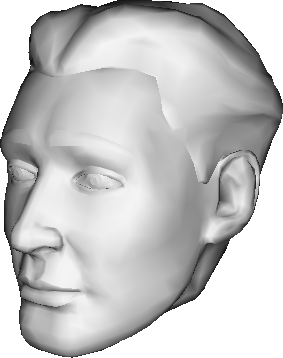
\includegraphics[width=4cm]{../images/cubehead_detail} &
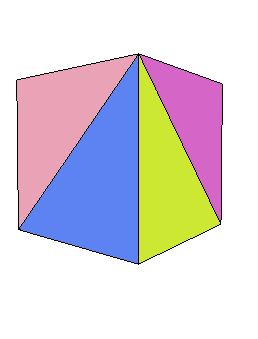
\includegraphics[width=4cm]{../images/cubehead_control_colour} &
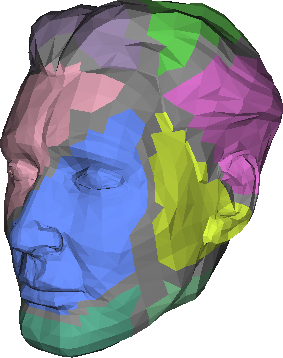
\includegraphics[width=4cm]{../images/cubehead_mapflat} \\
{\it (a)} & {\it (b)} & {\it (c)}
\end{tabular}
\begin{tabular}{cc}
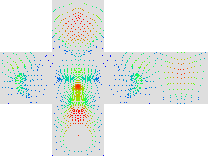
\includegraphics[width=5.9cm]{../images/cubehead_bigpoints} &
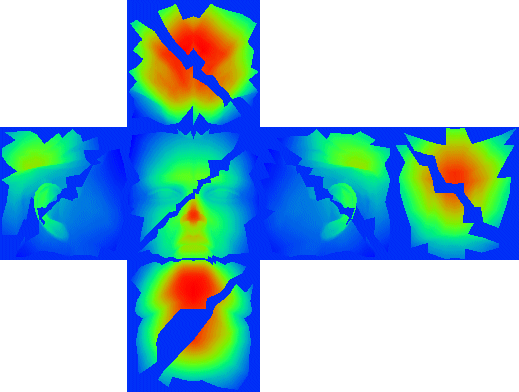
\includegraphics[width=5.9cm]{../images/cubehead_noedges} \\
{\it (d)} & {\it (e)} \\
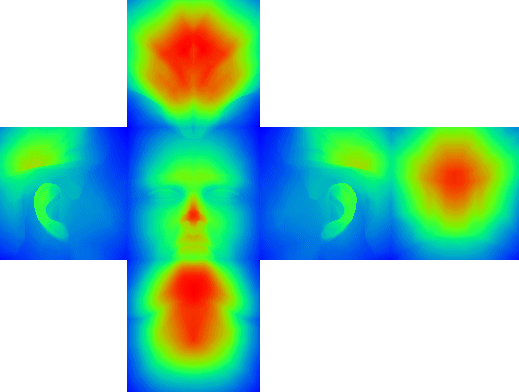
\includegraphics[width=5.9cm]{../images/cubehead_full} &
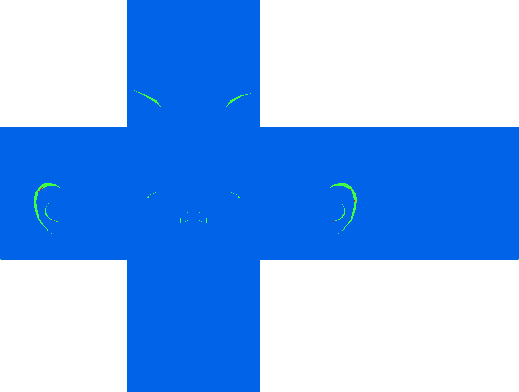
\includegraphics[width=5.9cm]{../images/cubehead_folds} \\
{\it (f)} & {\it (g)}
\end{tabular}
\caption[Displacement Mapping]{\label{fig:dispmap} Displacement Mapping Overview. (a) Original Mesh. (b) Control Mesh. (c) Mapping results. (see figure \ref{fig:detailmapping} for explanation of colour scheme). (d) Displacement map, points only. (e) Internal Triangles Filled. (f) Edge Triangles Filled. (g) Surface Folding. The displacement maps have been colourised to enhance the visibility of details.}
\end{center}
\end{figure}

In order to generate a displacement map representing the detail layer, we need to calculate the value of the error function across the surface of the control layer. To do this, we need to resample the 3D mesh from the detail layer into displacement values in a 2D image which is mapped to the control layer as described above. Conveniently, we have a simple way to do this from our previous calculations for layered animation. As explained in section \ref{sec:scandata:pointtosurface}, we represent each mapped detail layer vertex $\vec{p}$ as a set of four coordinates, $\omega_a$, $\omega_b$, $d$, and a control triangle index $t$.

This parameterisation will convert easily into an image-based format. If the control triangle $t_x$ has texture coordinates $\vec{u}_x\symbol{texcoord}$ for each of its vertices $\vec{v}_x$, then $\omega_a$ and $\omega_b$, the mapped coordinates of a detail layer vertex $\vec{p}$, define $\vec{u_{p}}$, a 2D position in the image for that point, as shown in equation \ref{eqn:imgpoint}.

\begin{equation} \label{eqn:imgpoint}
\vec{u_{p}} = \omega_a\vec{u}_a + \omega_b\vec{u}_b + (1-\omega_a-\omega_b)\vec{u}_c
\end{equation}

The distance value $d$ is then assigned to the pixel at this point. For the mesh shown in figure \ref{fig:dispmap}a (for which texture coordinates were assigned manually), the result of this process is shown in figure \ref{fig:dispmap}d. Each point in the image represents a point in the detail layer, and the colour of each point represents its distance. The texture image itself is composed of real-valued pixels at this stage, as we want to avoid losing any detail through quantisation until absolutely necessary.

\section{\label{sec:dispmapcreation:triangles}Filling Triangles}

While drawing the detail layer vertices into our displacement map may accurately encode all the vertex information from the detail layer, topological information (i.e. the mesh connectivity) is lost. When we create a displacement map, although we are not interested in the exact topology of the mesh, we do wish to preserve the exact shape of the detail layer surface. Therefore, rather than drawing individual points into the displacement map as described above, we calculate the displacement map over the {\it entire} detail layer surface by drawing complete detail layer triangles into the map.

Our triangle drawing method falls into two parts, that used for ${\cal T}^I$, and that used for ${\cal T}^E$. For each triangle $t \in {\cal T}^I$, we calculate a mapped triangle in the 2D image. This is done by mapping each of the detail layer triangle vertices into the image plane, creating a set of 2D coordinates for the vertices. These mapped points then form a triangle in the image which corresponds to the mapping of the detail layer triangle. The displacement values at the triangle vertices are taken directly from the detail layer mapping, but we must also calculate displacement values for every pixel inside the 2D mapped triangle.

\begin{figure}
\begin{center}
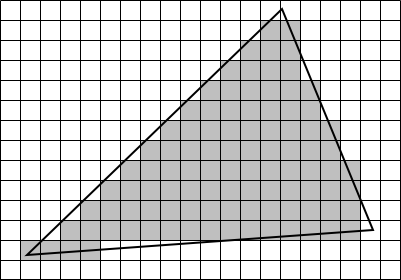
\includegraphics[width=6cm]{../images/raster}
\caption[Triangle Rasterisation]{\label{fig:raster} Triangle rasterisation identifies which pixel centres lie inside the triangle.}
\end{center}
\end{figure}

First of all, the mapped triangle is {\it rasterised}, a process in which we calculate which pixel centres lie inside the triangle boundary (see figure \ref{fig:raster}a). A set of areal coordinates $(\omega_a ,\omega_b ,\omega_c)$ are then calculated for each pixel centre $\vec{p}_x$ which lies inside the triangle $\triangle{\vec{u}_a,\vec{u}_b,\vec{u}_c}$. The areal coordinates are calculated using the area ratio method described in section \ref{sec:scandata:pointtosurface:areal}.

We can then use the areal coordinate for each pixel to calculate a displacement value $d_p$ for that pixel by barycentric interpolation of the displacement values $d_x$ at the corners $\vec{u}_x$ of the mapped triangle, which are obtained from the original point-to-surface mapping. 

\begin{equation} \label{eqn:pixeldisp}
d_p = \omega_a d_a + \omega_b d_b + \omega_c d_c
\end{equation}

In this way, each pixel whose centre lies within the triangle is filled with the appropriate interpolated displacement value. The results of this filling are shown in figure \ref{fig:dispmap}e. Note that at this stage, only triangles in ${\cal T}^I$ are filled.

A more efficient scanline conversion algorithm could be used instead of the per-pixel linear interpolation, but we choose to use the per-pixel calculation in the interests of keeping the algorithms generalised.

\subsection{\label{sec:dispmapcreation:triangles:approx}Linear Approximation}

\begin{figure}
\begin{center}
\begin{tabular}{cc}
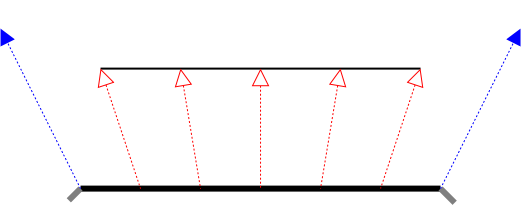
\includegraphics[height=3.5cm]{../images/approx_a} &
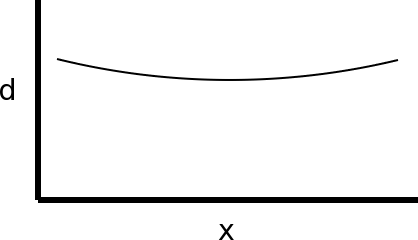
\includegraphics[height=3cm]{../images/approx_b} \\
{\it (a)} & {\it (b)} \\
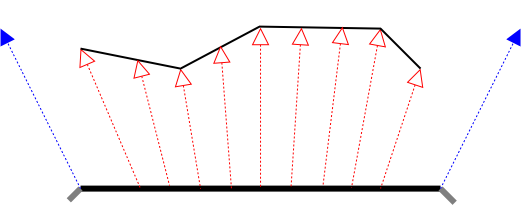
\includegraphics[height=3.5cm]{../images/approx_c} &
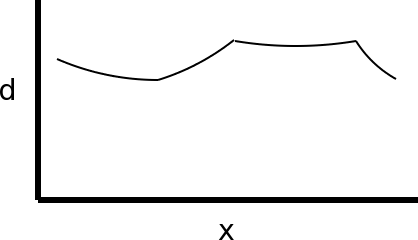
\includegraphics[height=3cm]{../images/approx_d} \\
{\it (c)} & {\it (d)} \\
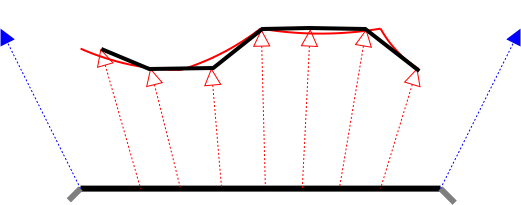
\includegraphics[height=3.5cm]{../images/approx_e} &
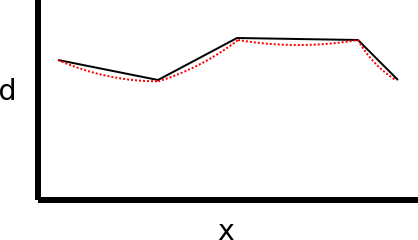
\includegraphics[height=3cm]{../images/approx_f} \\
{\it (e)} & {\it (f)}
\end{tabular}
\caption[Triangle Filling Approximation]{\label{fig:approximation} Triangle Filling Approximation. Examples shown in 2D for clarity. (a) A detail layer triangle maps to a control layer triangle. (b) d does not vary linearly. (c) Comparatively small triangles map to a control layer triangle. (d) Approximation error is reduced as triangles become smaller. (e) Sampling and quantisation errors. (f) Linear approximation. }
\end{center}
\end{figure}

The linear interpolation across detail layer triangles, described above, does not in fact represent the surface shape with full accuracy, but includes a linear approximation which simplifies calculation of the displacement map.

Figure \ref{fig:approximation}a shows 2D representation of a detail layer triangle, of a similar size to the control layer triangle it is being mapped to. Due to the shape of the normal volume and the mapping between layers, the distance between each point on the surface of the detail triangle and its mapping to the control surface will vary across the triangle, even if the two are parallel. 

Figure \ref{fig:approximation}b shows how the $d$ value varies across the surface. The distance is not only related to the position of the detail layer surface, but also to the angle formed between the mapping vector and the control layer triangle at the point in question. If we represent the displacement values across a triangle by a linear interpolation, errors will be introduced as we fail to capture the curvature shown in figure \ref{fig:approximation}b correctly.

The situations shown in figure \ref{fig:approximation}a will be rare, as detail layer triangles will normally be substantially smaller than the control layer triangles that they are mapped to, as shown in figure \ref{fig:approximation}c. In this case, the surface is formed of many detail layer triangles across the surface of the control triangle, each of which is curved in normal volume space as shown in figure \ref{fig:approximation}d. As they are explicitly calculated, the displacement values at vertices on the detail layer will always be correct, meaning that the error introduced by our linear interpolation is reduced, as the surface is ``fixed'' to the correct displacement value at each vertex. Our linear approximation will lie much closer to the actual surface shape as shown in figure \ref{fig:approximation}f.

The errors introduced by this linear approximation are acceptable however, as they are only significant at certain scales, and in the remainder of cases will be insignificant compared to other sources of error. Firstly, errors will only be significant when a detail layer triangle fills a large proportion of the normal volume in which it lies. As we are generally mapping very dense meshes to much simpler control layers, this should be an exceptional case and occur only rarely. Secondly, processes which take place after the creation of the displacement map, for instance quantisation for file storage, or resampling for detail layer reconstruction, will introduce further errors and approximations which will dominate over the small scale of these linear approximation errors.

For these reasons, and because it simplifies the method and reduces computation time during map creation, we accept this linear approximation as part of our method. It would be entirely possible to remove this error by using a more complex method of triangle-filling, if it became necessary to remove such errors for any particular application. For instance, the errors may become visible in a highly detailed rendering, or under strong specular lighting which may cause the surface to appear dimpled.

\section{\label{sec:dispmapcreation:edges}Dealing with Edge Triangles}
\begin{figure}
\begin{center}
\begin{tabular}{cccc}
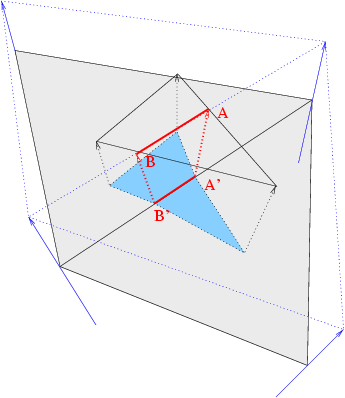
\includegraphics[height=5cm]{../images/edgetriangle_b} &
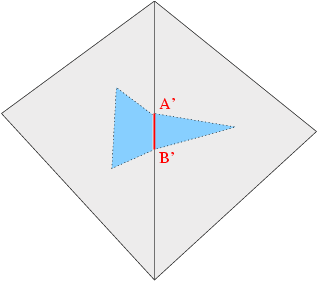
\includegraphics[height=5cm]{../images/edgetriangle_a} \\
{\it (a)} & {\it (b)} \\
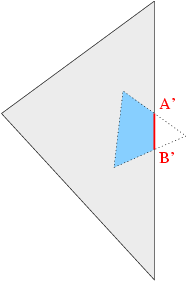
\includegraphics[height=5cm]{../images/edgetriangle_c} &
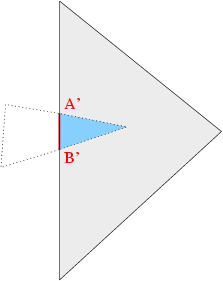
\includegraphics[height=5cm]{../images/edgetriangle_d} \\
{\it (c)} & {\it (d)}
\end{tabular}
\caption[Edge Triangles]{\label{fig:edgetriangles} Edge Triangles that lie across normal volume boundaries may become non-triangular when projected to a 2D plane.}
\end{center}
\end{figure}
\begin{figure}
\begin{center}
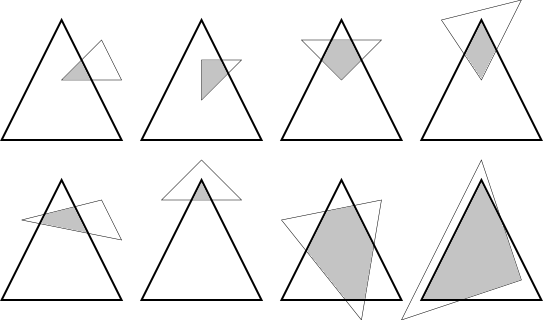
\includegraphics[width=8cm]{../images/edgetris}
\caption[Edge Cases]{\label{fig:edgecases} Edge Cases. A selection of the possible configurations of the intersection between a control triangle and a detail layer triangle. The area that must be filled is shaded.}
\end{center}
\end{figure}
The method described above suffices for generating displacement map data for triangles in ${\cal T}^I$. However, for those triangles in ${\cal T}^E$, whose vertices map to two or more control mesh triangles, the situation becomes more complex. Even though it is the case that for triangles in ${\cal T}^I$, a triangle will remain triangular when mapped to the 2D image, it is not the case for edge triangles. 

A triangle is mapped linearly inside each normal volume onto the appropriate control triangle. However, adjacent normal volumes will have different mapping properties. This means that if a detail layer triangle crosses a normal volume boundary (as shown in figure \ref{fig:edgetriangles}a), the linear mapping of the triangle will have different parameters on either side of the boundary. The triangle will therefore not remain triangular when mapped to the image plane, as shown in figure \ref{fig:edgetriangles}b.  Therefore, we have to treat the mapping to each control triangle entirely separately, even in cases where edges are shared in the image plane.

For each triangle $t_e \in {\cal T}^E$, we separately calculate its projection into each triangle whose normal volume it crosses. This is not limited to those triangles which its vertices map to, as it may completely cross a normal volume without any of its vertices mapping to the appropriate control triangle. The intersection can take many shapes, some examples of which are shown in figure \ref{fig:edgecases}. Detecting all of the potential cases and filling the displacement map with the appropriate values can be a complex process. This section will discuss the methods we have used for this purpose.

\subsection{\label{sec:dispmapcreation:edges:virtual}Virtual Corner Points}

Initially, in an attempt to avoid calculating the sections of the detail triangle inside each normal volume, a class of drawing methods were explored that involved extending the point-to-surface mapping beyond the normal volume boundary. In order to draw a point into the image plane, we need to calculate its $\omega_a$, $\omega_b$ and $d$ coordinates for the control triangle currently being drawn. In these methods, we calculate these parameters for all detail layer points that are used by an edge triangle, including those that were not originally mapped to the control triangle in question. These calculated points are referred to herein as {\it virtual corner points}.

There were a number of problems with these methods, however. The mapping outside the normal volume proved to be highly unstable, some methods involved time-consuming searches, and all of the methods resulted not in a general algorithm for drawing, but instead a large number of special cases, each of which had to be implemented separately. Therefore, alternative approaches were explored, involving explicit calculation of the triangle sections inside each normal volume. 

%The virtual corner point methods are explained in more detail in appendix \ref{sec:edgemethods}, as although they are not directly related to the final method used, they may still be of some interest. 

\subsection{\label{sec:dispmapcreation:edges:intersection}Intersection Calculation}

If we are to calculate the shape of edge triangles, we must calculate the intersections between the edges of the detail layer edge triangle, and the normal volume boundary of the control triangle we wish to draw it into. However, this is not a simple operation, because the boundaries of the normal volume are not planar, but bilinear ruled surfaces, as mentioned in section \ref{sec:scandata:normalvolume:boundaries}. We therefore use the following method to calculate the intersections with this surface.

Any point $\vec{r}_e$ which lies on an edge of a detail layer triangle can be defined as shown in equation \ref{eqn:intersect_edge}, where $\vec{p}_0$ and $\vec{p}_1$ are the vertices at either end of the detail triangle edge in question, and , and $0 \leq \kappa \leq 1$.

\begin{equation} \label{eqn:intersect_edge}
\vec{r}_e = \kappa\vec{p}_0 + (1-\kappa)\vec{p}_1
\end{equation}

In a similar way, a point $\vec{r}_b$ which lies on a normal volume boundary can be defined as shown in equation \ref{eqn:intersect_boundary}. $\hat{n}_x$ is the surface normal at the control triangle vertex $\vec{v}_x$, $\vec{v}_0$ and $\vec{v}_1$ represent the control triangle vertices at the either end of the normal volume boundary we are testing, and $0 \leq \lambda \leq 1$.

\begin{equation} \label{eqn:intersect_boundary}
\vec{r}_b = \lambda\vec{v}_0 + (1-\lambda)\vec{v}_1 + d(\lambda\hat{n}_0 + (1-\lambda)\hat{n}_1)
\end{equation}

As the intersection point will lie on both the detail triangle edge and the normal volume boundary, the intersection point $\vec{r} = \vec{r}_e = \vec{r}_b$.

Combining equations \ref{eqn:intersect_edge} and \ref{eqn:intersect_boundary} gives us a single equation describing the intersection point, in terms of the unknown values $\lambda$, $\kappa$, and $d$. This formulation is illustrated in figure \ref{fig:intersection}.

\begin{equation} \label{eqn:intersect_combined}
\vec{r} = \kappa\vec{p}_0 + (1-\kappa)\vec{p}_1 = \lambda\vec{v}_0 + (1-\lambda)\vec{v}_1 + d(\lambda\hat{n}_0 + (1-\lambda)\hat{n}_1)
\end{equation}

\begin{figure}
\begin{center}
\setlength{\unitlength}{0.5cm}
\begin{picture}(14,12)
% Points
\put(0,4){\circle*{0.2}}
\put(6,10){\circle*{0.2}}
\put(8,2){\circle*{0.2}}
\put(14,8){\circle*{0.2}}
\put(4,5){\circle*{0.2}}
\put(7,6){\circle*{0.2}}
\put(10,7){\circle*{0.2}}
% Lines
\thinlines
\put(0,4){\line(1,1){6}}
\put(6,10){\line(4,-1){8}}
\put(0,4){\line(4,-1){8}}
\put(8,2){\line(1,1){6}}
\put(6,10){\line(1,-4){2}}
\put(4,5){\line(3,1){6}}
% Normals
\put(6,10){\vector(1,1){2}}
\put(8,2){\vector(-1,-2){1}}
% Labels
\put(3,4.5){$\vec{p}_0$}
\put(10.5,7){$\vec{p}_1$}
\put(5,10){$\vec{v}_0$}
\put(8,1){$\vec{v}_0$}
\put(8,11){$\hat{n}_0$}
\put(6,0){$\hat{n}_1$}
\put(7.5,5.5){$\vec{r}$}
\put(5,5.75){$\kappa$}
\put(7,7.5){$\lambda$}
\end{picture}
\caption[Intersection Calculations]{\label{fig:intersection} Intersection Calculations. Parameters used in the calculation of the intersection point $\vec{r}$ between a line segment and a normal volume boundary. }
\end{center}
\end{figure}

This formula can then be then solved for the three unknowns, $\lambda$, $\kappa$ and $d$, using the following method. First, we define some useful symbols:
\begin{eqnarray}
\vec{p}_{01} & = & \vec{p}_0 - \vec{p}_1 \nonumber \\
\vec{v}_{01} & = & \vec{v}_0 - \vec{v}_1 \nonumber \\
\vec{n}_{01} & = & \hat{n}_0 - \hat{n}_1 \nonumber
\end{eqnarray}

Rearranging equation \ref{eqn:intersect_combined}:

\begin{equation} \label{eqn:intsolv0}
\vec{p}_1 + \kappa\vec{p}_{01} = \vec{v}_1 + d\hat{n}_1 + \lambda(\vec{v}_{01}+d\vec{n}_{01})
\end{equation}

Using the facts that $\vec{a} \times \vec{a} = \vec{0}$ and $d\vec{a} \times \vec{b} = d(\vec{a} \times \vec{b})$, we now take the cross product of both sides with $\vec{p}_{01}$ in order to remove the $\kappa$ component:

\begin{equation}
\vec{p}_1 \times \vec{p}_{01} = (\vec{v}_1 + d\hat{n}_1) \times \vec{p}_{01} + \lambda(\vec{v}_{01}+d\vec{n}_{01}) \times \vec{p}_{01}
\end{equation}
\begin{equation} \label{eqn:intsolv1}
(\vec{p}_1 - \vec{v}_1 - d\hat{n}_1) \times \vec{p}_{01} = \lambda(\vec{v}_{01}+d\vec{n}_{01}) \times \vec{p}_{01}
\end{equation}

We now use the property that $(\vec{a} \times \vec{b}) \cdot \vec{a}  = 0$ to remove $\lambda$ from the equation, leaving only $d$ to solve for.

\begin{equation}
((\vec{p}_1 - \vec{v}_1 - d\hat{n}_1) \times \vec{p}_{01}) \cdot (\vec{v}_{01}+d\vec{n}_{01}) = 0
\end{equation}
\begin{eqnarray} \label{eqn:intsolv2} 
d^2((\hat{n}_1 \times \vec{p}_{01}) \cdot \vec{n}_{01})  & + & \nonumber \\
d((\hat{n}_1 \times \vec{p}_{01} \cdot \vec{v}_{01}) + (\vec{v}_1 \times \vec{p}_{01} \cdot \vec{n}_{01}) - (\vec{p}_1 \times \vec{p}_{01} \cdot \vec{n}_{01})) & + & \nonumber \\
(\vec{v}_1 \times \vec{p}_{01} \cdot \vec{v}_{01}) - (\vec{p}_1 \times \vec{p}_{01} \cdot \vec{v}_{01}) & = & 0
\end{eqnarray}

Equation \ref{eqn:intsolv2} is a quadratic in $d$, and so can be solved using standard methods. The real roots of this equation represent the value of $d$ for potential intersection points. We can now use each possible value of $d$ to calculate possible values for $\lambda$ and $\kappa$. First of all, we can rearrange equation \ref{eqn:intsolv1} for $\lambda$:

\begin{equation} \label{eqn:lambda}
\lambda = \frac{((\vec{p}_1 - \vec{v}_1 - d\hat{n}_1) \times \vec{p}_{01}) \cdot (\vec{v}_{01}+d\vec{n}_{01} \times \vec{p}_{01})}{\|(\vec{v}_{01}+d\vec{n}_{01} \times \vec{p}_{01})\|^2}
\end{equation}

We can then rearrange equation \ref{eqn:intsolv0} to calculate the corresponding value of $\kappa$.

\begin{equation} \label{eqn:kappa}
\kappa = \frac{(\vec{v}_1 + d\hat{n}_1 + \lambda(\vec{v}_{01}+d\vec{n}_{01}) - \vec{p}_1) \cdot \vec{p}_{01}}{\|\vec{p}_{01}\|^2}
\end{equation}

After the calculation is complete, we can discard some potential solutions, as they are outside the desired range. As mentioned above, both $\lambda$ and $\kappa$ must lie between 0 and 1 for the intersection to be valid. The above method may yield results outside that range, in which case they are discarded.

This intersection calculation was developed by Gordon Collins.

\subsection{\label{sec:dispmapcreation:edges:polygon}Polygon Creation}

Once we can detect intersection points between detail layer edges and normal volume boundaries, we can use this information to calculate the exact geometric intersection of the detail triangle and all of the normal volumes in which it lies. Due to the nature of the intersection method, the mapping of this triangle to the control triangle is performed in the same operation as the intersection calculation, so a 3D intersection is never calculated, and the results of the calculation enable us to draw the displacement map directly.

To draw a detail layer triangle into the area of a displacement map  corresponding to a control layer triangle, we calculate a polygon with up to six sides (as shown in figure \ref{fig:edgecases}), which represents the geometric intersection of the detail layer triangle and the normal volume of the control layer triangle. Each point in the polygon is represented by a 2D image plane coordinate, and an associated displacement value. The problem of filling such an arbitrary polygon is discussed below in section \ref{sec:dispmapcreation:edges:filling}.

To build this polygon, we treat each edge of the detail layer triangle in turn. Firstly, we examine the starting vertex of the edge. If the vertex maps to the current control triangle, we add the texture coordinate of the vertex to the polygon, along with its associated displacement value. Then, we examine the ending vertex of the edge. If this also maps, we add it to the polygon as before and proceed to the next edge. Otherwise, we detect intersections between the edge and all boundaries of the normal volume. In this case, there should be only one in the correct range. We add this intersection to the polygon. Its texture coordinate values are interpolated from the end points of the normal volume boundary using the $\lambda$ result of the intersection calculation above. The displacement value, $d$, for the point is obtained directly from the solution to the intersection calculation.

If the starting vertex does not map to the current control triangle, we proceed directly to the calculation of the intersection point. In this case, we can obtain either 0, 1 or 2 results. If there are no results, we proceed directly to the next detail edge - this edge does not cross the normal volume. Otherwise, both intersections are added to the polygon as before, in order of increasing $\kappa$ (which corresponds to a distance along the detail triangle edge).

The only addition to this comes when an incoming edge is detected (i.e. the start point is outside the volume, and intersections are found). In this case we must detect whether the last outgoing edge was on the same side of the normal volume. If not, then we must include all corners of the control triangle between the two edges in our polygon. This involves explicitly calculating a displacement value for the corner point, by using a ray/triangle intersection method.

Once we can draw into a single control triangle, it is a simple matter to draw into many. Starting with each corner point, we maintain a {\it todo} list of normal volumes (identified by their associated control triangle) that we know the detail layer triangle crosses. For each of these, we carry out the method described above. If we detect that the triangle intersects a normal volume boundary, then the normal volume on the other side of that boundary is added to the {\it todo} list. Once drawing is complete in a normal volume, then that volume is added to a {\it done} set. Then, the next volume on the {\it todo} list is processed, as long as it is not in the {\it done} set. Using this method, we will walk around the control layer mesh until the entire detail triangle surface has been drawn into the displacement map.

\begin{algorithm}[tbp]
\begin{algorithmic}
\STATE add detail layer vertex mappings to control triangle todo list
\FORALL { triangle $t$ in todo list}
	\FORALL {edge $e_i \in {\cal E}$ }
		\IF {$v_i$ maps to this control triangle}
			\STATE append $v_i$ to the corner list
			\IF {$v_{i+1}$ does not map to this control triangle}
				\STATE detect intersections between $e_i$ and normal volume boundaries
				\STATE sort intersections into order of lowest $\kappa$
				\STATE append first intersection to corner list
				\STATE {\em LastBoundary} $\Leftarrow$ intersected boundary
				\IF {triangle over intersected boundary is not on done list}
					\STATE add triangle over intersected boundary to todo list
				\ENDIF
			\ENDIF
		\ELSE
			\STATE detect intersections between $v_i$ and normal volume boundaries
			\IF {there are any intersections}
				\STATE sort intersections into order of lowest $\kappa$
				\IF {intersected boundary $\neq$ {\em LastBoundary}}
					\STATE append all control triangle corners between this boundary and the last to the corner list
				\ENDIF
				\STATE append the first intersection to the corner list
				\IF {$v_{i+1}$ does not map to this control triangle}
					\STATE append the second intersection to the corner list
					\STATE {\em LastBoundary} $\Leftarrow$ intersected boundary
					\IF {triangle over intersected boundary is not on done list}
						\STATE add triangle over intersected boundary to todo list
					\ENDIF
				\ENDIF
			\ENDIF
		\ENDIF
	\ENDFOR
	\STATE add $t$ to done list
\ENDFOR
\end{algorithmic}
\caption{\label{alg:polygoncreation}Polygon Generation}
\end{algorithm}

The complete process is summarised in algorithm \ref{alg:polygoncreation}.

\subsection{\label{sec:dispmapcreation:edges:filling}Filling of Non-Triangular Polygons}

It is simple to interpolate values across a triangular region, as explained in section \ref{sec:dispmapcreation:triangles}, but this barycentric interpolation method does not extend directly to polygons with more than 3 sides, as it is not a simple matter to calculate areal coordinates for arbitrary polygons. However, \citet{Meyer02} describe a simple method of generalising areal coordinates to irregular convex polygons, which we can use to fill our clipped triangles. 

This method calculates an areal coordinate for every vertex of an irregular polygon, and preserves the properties found in standard areal coordinates for triangles. A point inside the polygon is represented as an affine combination of the vertices weighted by their areal components, and the sum of all the areal coordinates is 1 for a point inside. The parameterisation is also continuous in all its derivatives, guaranteeing smoothness of the interior under animation of the polygon vertices.

To obtain the $i$th areal coordinate for a point $\vec{p}_x$, we use the formulation shown in equation \ref{eqn:nontriareals}. $\vec{v}_i$ represents the $i$th vertex of the enclosing polygon.
\begin{eqnarray}
\label{eqn:nontriareals}
\vec{v}_p & = & \vec{p}_x - \vec{v}_i \nonumber \\
\vec{v}_- & = & \vec{v}_{i-1} - \vec{v}_i \nonumber \\
\vec{v}_+ & = & \vec{v}_{i+1} - \vec{v}_i \nonumber \\
\theta_- & = & \frac{\vec{v}_- \cdot \vec{v}_p}{\| \vec{v}_- \times \vec{v}_p \|} \nonumber \\
\theta_+ & = & \frac{\vec{v}_+ \cdot \vec{v}_p}{\| \vec{v}_+ \times \vec{v}_p \|} \nonumber \\
\omega_i & = & \frac{\theta_- + \theta_+}{\| \vec{v}_p \| ^2}
\end{eqnarray}

The calculated areal coordinates are then used to calculate the distance value $d_x$ at $\vec{p}_x$ in a similar way to that for triangle filling. $d_i$ represents the distance value at $\vec{v}_i$.

\begin{equation}
\label{eqn:polygonfilling}
d_x = \sum_{i=1}^n \omega_id_i
\end{equation}

\section{\label{sec:dispmapcreation:raycasting}Raycasting}

There is an alternative method of generating the displacement map from that presented above, involving {\it raycasting}. Once the texture coordinates are generated for the control mesh, this method would calculate the 3D position of each pixel in the displacement map on the surface of the control layer. A ray would then be cast along the interpolated surface normal at that point, and any intersections with the detail layer found directly. The distance between the control layer point and the detail layer intersection point would then be stored in the displacement map. 

This technique is perfectly valid, and simpler than the one we present above. It also avoids the linear approximation problem noted in section \ref{sec:dispmapcreation:triangles:approx}, giving a more accurate result. However, one advantage of our approach is that a raycasting approach would need to be specifically designed to cope with holes in the detail mesh, as well as boundaries and so on. Our approach avoids this, as it calculates displacements for each point on the detail mesh, not for each point on the control mesh.

Another advantage of our method is that it should be faster to execute. This is because a raycasting approach must search for intersections between the ray and the detail layer by testing each detail layer triangle in turn. Our approach uses existing mapping results, and fills pixel values in the displacement map directly from these, with no searching required. This implies that the triangle filling method has a lower order than the raycasting method, making it more efficient.

\section{\label{sec:dispmapcreation:folding}Surface Folding}

One problem with scalar-valued displacement maps is that if the mapping from high resolution model to low resolution control layer is non-injective, data loss can occur since the mapping is no longer invertible. If the high resolution model folds over itself inside the normal volume of a single control triangle, a single point on the surface of that control triangle will have more than one possible displacement value. This is an inherent limitation in the displacement mapping process, and cannot be solved except by recreation of the control layer, removing the non-injective areas. As mentioned earlier in section \ref{sec:scandata:creation:control}, this condition can be enforced during automatic control layer generation.

If this undesirable situation does arise (perhaps because we are not automatically generating a control model, therefore cannot force injectivity), we choose to store whichever displacement value is the highest (i.e. most positive). This will give a correct reconstruction for the outer surface of the detail layer, while the folded surface will be lost. However, these surfaces will tend to be less visible anyway, so the aesthetic impact of these situations is kept to a minimum. Figure \ref{fig:dispmap}g shows surface folding for the displacement map shown in figure \ref{fig:dispmap}f. Each pixel is coloured according to the number of times it is "hit" (i.e. drawn onto).

\section{\label{sec:dispmapanim:reconstruction}Surface Reconstruction}

Once the layered model has been created and stored in the appropriate manner, at some point it will need to be displayed. Interactive rendering systems are currently incapable of direct rendering of displacement maps, so in order to display the resulting model we must convert it back into a standard polygon mesh. In order to do this, we subdivide the control layer mesh, creating a new version of the control mesh which contains more polygons than the original, which can represent a more complex surface. The vertices which are introduced by this subdivision process will initially lie on the surface of the control mesh. However, we then displace each vertex along the interpolated control mesh normal at that point. The amount of this displacement is determined by sampling the displacement map at the appropriate point and multiplying the normal at that point by the resulting value.

\subsection{\label{sec:dispmapanim:reconstruction:subdivision}Control Layer Subdivision}

The first stage in the process of rebuilding the surface detail from a displacement map is to subdivide the control layer to the desired level, so that the detail from the displacement map can be represented by the mesh. A number of subdivision methods were reviewed in section \ref{sec:litreview:surfaces:smooth:subdivision}. However, we do not wish to generate a smooth surface from our polygon mesh, as the displacements were measured from the piecewise linear control mesh surface. We therefore use simpler subdivision approaches that perform no smoothing and simply subdivide the surface without changing its geometry. We can use a simple uniform subdivision method to refine the entire surface equally, but this may involve calculating and rendering parts of the model that are not required, so we can also use adaptive subdivision techniques, where different parts of the model are subdivided to different levels.

\subsubsection{\label{sec:dispmapanim:reconstruction:subdivision:uniform}Uniform Subdivision}
\begin{figure}
\begin{center}
\begin{tabular}{ccccc}
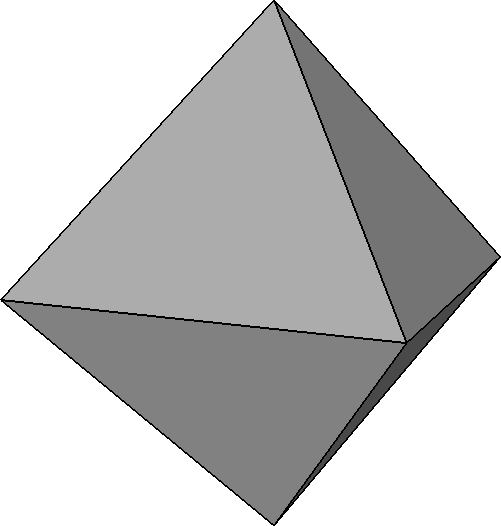
\includegraphics[width=2.5cm]{../images/level0} &
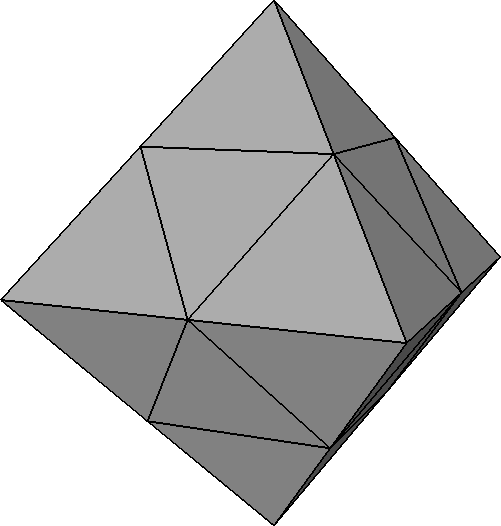
\includegraphics[width=2.5cm]{../images/level1} &
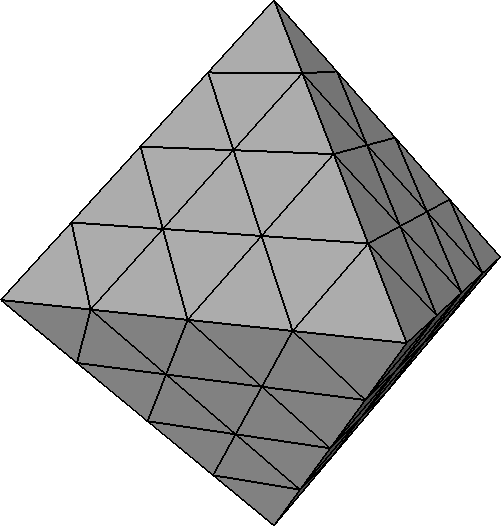
\includegraphics[width=2.5cm]{../images/level2} &
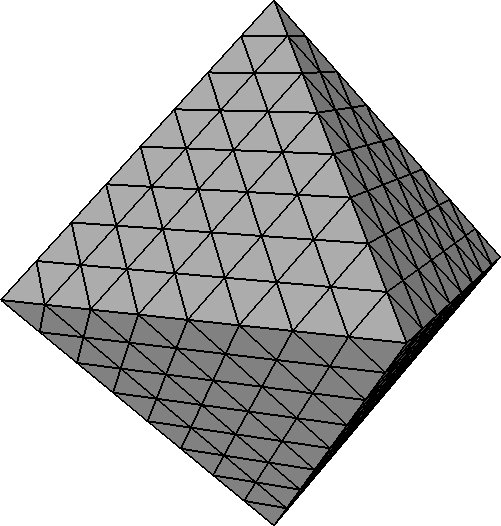
\includegraphics[width=2.5cm]{../images/level3} &
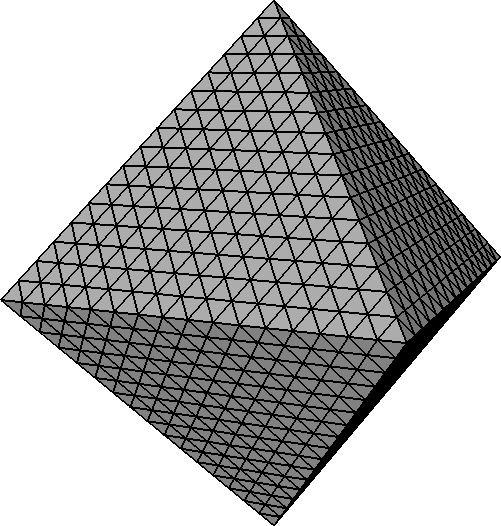
\includegraphics[width=2.5cm]{../images/level4} \\
\end{tabular}
\caption[Uniform Subdivision]{\label{fig:uniformsubdiv} Uniform Subdivision, showing levels 0 to 4. Each level contains four times as many polygons as the last. }
\end{center}
\end{figure}

In \cite{Smith00a}, we presented an algorithm for the efficient calculation of a uniform quaternary subdivision of a triangle mesh, developed by Wei Sun. The algorithm recursively generates four subdivided triangles for each original triangle, adding a new vertex to the midpoint of each mesh edge, as illustrated in figure \ref{fig:uniformsubdiv}. The new vertices are created as areal coordinates $\omega_a$ and $\omega_b$ relative to their enclosing control layer triangle. 3D positions for all vertices can then be calculated from these parameters as explained below in section \ref{sec:dispmapanim:reconstruction:sampling}.

As each level of subdivision introduces multiplies the number of triangles by four, the triangle count for each level is $t_c \times 4^l$, where $l$ is the level of subdivision, and $t_c$ is the number of triangles in the original mesh.

\subsubsection{\label{sec:dispmapanim:reconstruction:subdivision:adaptive}Adaptive Subdivision}

Another possibility is to subdivide the mesh adaptively, refining the surface only in those areas in which we are most interested. This method has the advantage that displacements are not calculated where they are not required, and polygons are used as efficiently as possible, keeping rendering time to a minimum. Areas of interest, where we wish to subdivide the mesh, can be defined in a number of ways.

View-based adaptive subdivision would refine the mesh in areas based on the direction in which the viewer is looking. Subdivision could be performed only in regions which are visible to the user without wasting polygons on invisible regions. It would also be possible to refine the geometry purely around the outline of the mesh as observed by the viewer, so that the silhouette of the mesh is realistic. If the surface inside the silhouette is textured as well as displacement mapped, this may provide a reasonably realistic appearance.

Subdivision could also be adaptive based on curvature of the control mesh. In this case, refinement would take place more in areas where the control layer is curved, and less so on flat regions. However, subdivision may not be performed in areas where fine surface details are present on locally flat regions of the control layer, meaning that this fine detail is lost. Also, this is only useful if the control layer is sufficiently detailed as to provide meaningful curvature information that varies across the mesh. 

Another approach would be to subdivide based on the actual values in the displacement map. Subdivision could be based either on the total error between the surfaces (i.e. more subdivision in areas with higher displacement values), or based on the gradient of the displacement values. The gradient of the image directly relates to curvature of the detail layer mesh, so a subdivision scheme based on this would give the optimal reconstruction of surface details.

All of these methods may provide interesting and potentially useful results. However, the scope of this research has not allowed further investigation, and as such they will not be expanded upon further. We restrict ourselves only to uniform reconstruction of displacement maps as discussed above.

\subsection{\label{sec:dispmapanim:reconstruction:sampling}Vertex Position Calculation}

Once the control mesh has been subdivided to give the level of detail required, we need to refine the shape of the new subdivided mesh so that it follows the shape of the original detail layer. After application of the subdivision algorithm above, the mesh consists of a set of vertices in the form ($\omega_a$, $\omega_b$, $t$). From these parameters, we can calculate a 3D position for each subdivided vertex as follows. 

Firstly, we must calculate the position $\vec{p}_x$ of each subdivided vertex $x$ on the surface of the control mesh. This can be calculated by simple linear interpolation of the vertices of the control mesh triangle $t$.

\begin{equation}
\vec{p}_x = \omega_a \vec{v}_{ta} + \omega_b \vec{v}_{tb} + (1 - \omega_a - \omega_b) \vec{v}_{tc}
\end{equation}

We can also calculate the interpolated normal at the point $\vec{p}_x$ by a similar linear interpolation of the normals at the vertices of the triangle $t$.

\begin{equation}
\vec{n}_x = \omega_a \hat{n}_{ta} + \omega_b \hat{n}_{tb} + (1 - \omega_a - \omega_b) \hat{n}_{tc}
\end{equation}

The final 3D position $\vec{v}_x$ of the vertex $x$ will lie along the line $\vec{p}_x + d\vec{n}_x$. The distance along this line $d$ is the displacement value that we have calculated previously, and must be recovered from the displacement map. The triangle $t$ has a set of three image coordinates, one for each of its vertices, ($\vec{u}_{ta},\vec{u}_{tb},\vec{u}_{tc}$). The image coordinate $\vec{u}_x$ of the subdivided vertex $\vec{v}_x$ can be calculated by linear interpolation between these coordinates as shown in equation \ref{eqn:calcpixel}.

\begin{equation} \label{eqn:calcpixel}
\vec{u}_x = \omega_a \vec{u}_{ta} + \omega_b \vec{u}_{tb} + (1 - \omega_a - \omega_b) \vec{u}_{tc}
\end{equation}

This gives us the image coordinate of the correct displacement sample, whose value $d$ will be the displacement value for the vertex $x$. Obviously, the sample point will rarely lie precisely on the centre of a pixel, so the displacement value is taken from the pixel whose centre is closest to the sample point.

When the distance value has been recovered, we can calculate the final vertex position $\vec{v}_x$.

\begin{equation}
\vec{v}_x = \vec{p}_x + d \vec{n}_x
\end{equation}

This reconstruction process is carried out for each vertex in the subdivided mesh. The results of performing this reconstruction operation for an entire mesh are shown in the next section. Each progressive level of subdivision adds more detail from the displacement map, until the regenerated mesh is visually indistinguishable from the original.

\section{\label{sec:dispmapcreation:lmtool}LMTool Interface}
\begin{figure}
\begin{center}
\begin{tabular}{cccc}
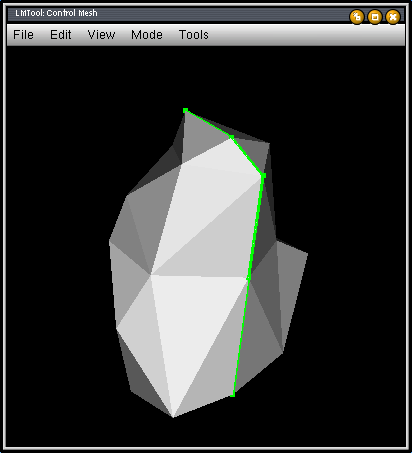
\includegraphics[width=3.5cm]{../images/lmtool_pelting} &
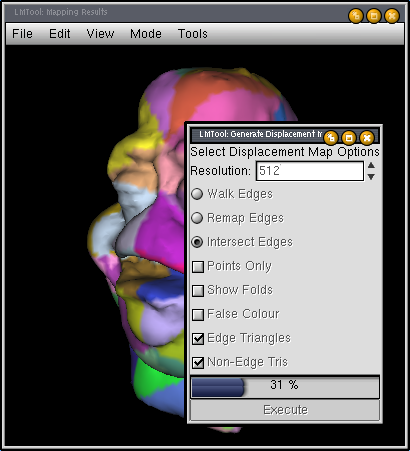
\includegraphics[width=3.5cm]{../images/lmtool_dispmapdialog} &
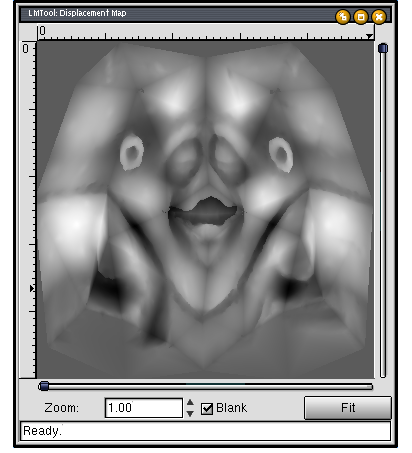
\includegraphics[width=3.5cm]{../images/lmtool_dispmap} &
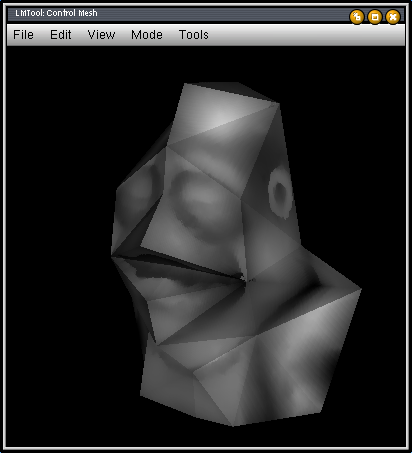
\includegraphics[width=3.5cm]{../images/lmtool_dispmaptexture} \\
{\it(a)} & {\it(b)} & {\it(c)} & {\it(d)} 
\end{tabular}
\caption[LMTool Displacement Mapping]{\label{fig:lmtooldispmap} LMTool Displacement Mapping. The screenshots show the process of generating a displacement map from a mapped detail layer. (a) Seams are defined across the back of the Monster head model to generate a pelt. (b) A displacement map is generated. (c) The resulting map is displayed in 2D, and (d) also displayed as a texture map on the control model.}
\end{center}
\end{figure}
The LMTool application introduced in section \ref{sec:scandata:creation:lmtool} also provides support for the creation of displacement maps. The program allows the user to define seams on the control model (shown in figure \ref{fig:lmtooldispmap}a), which are used to split the mesh, allowing creation of a pelted displacement map as described above in section \ref{sec:dispmapcreation:unwrap}.

Once a mapping has been calculated as described in chapter \ref{sec:scandata}, the program provides the option to generate a displacement map, using the dialog shown in figure \ref{fig:lmtooldispmap}b. The user can select a size for the resulting displacement image, and select from a number of rendering options, mainly used for testing and debugging. The user then presses ``Execute'' to start the displacement mapping process. Once the map is created, it is displayed both as a 2D image (shown in figure \ref{fig:lmtooldispmap}c) and as a texture map on the surface of the control layer, as shown in figure \ref{fig:lmtooldispmap}d.

The program also has the capability to rebuild a detailed surface from a displacement map representation, using a uniform subdivision method. The user simply selects the required level of subdivision from a menu, and the model is regenerated to that level and displayed.

\section{\label{sec:dispmapcreation:results}Results}

\begin{figure}
\begin{center}
\begin{tabular}{cc}
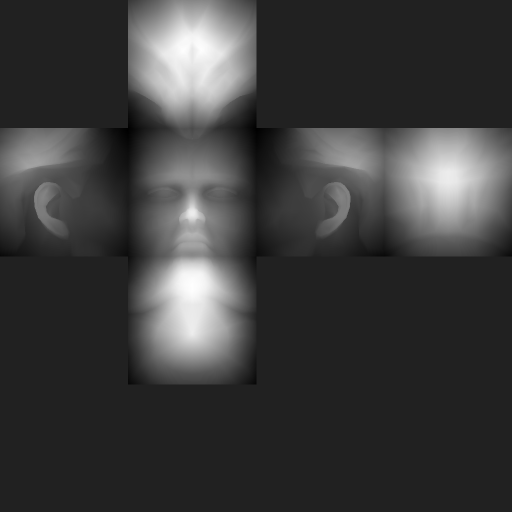
\includegraphics[width=6cm]{../images/dispmap_cubehead} &
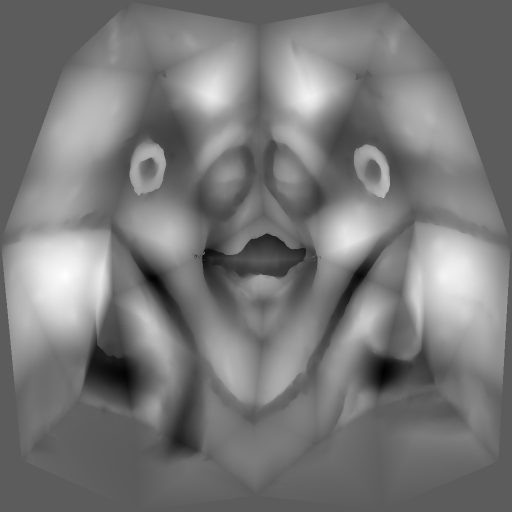
\includegraphics[width=6cm]{../images/dispmap_dinohead} \\
{\it (a)} & {\it (b)} \\
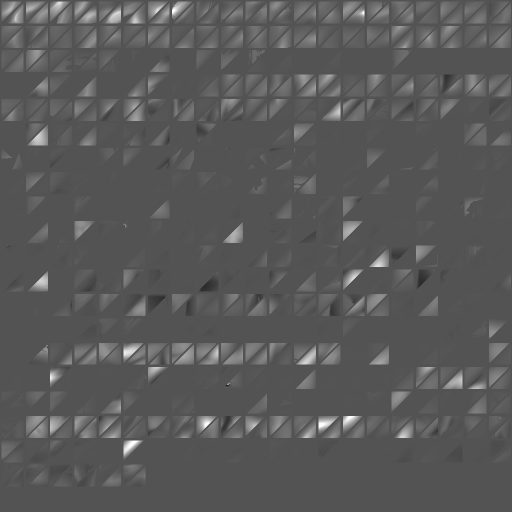
\includegraphics[width=6cm]{../images/dispmap_horse} &
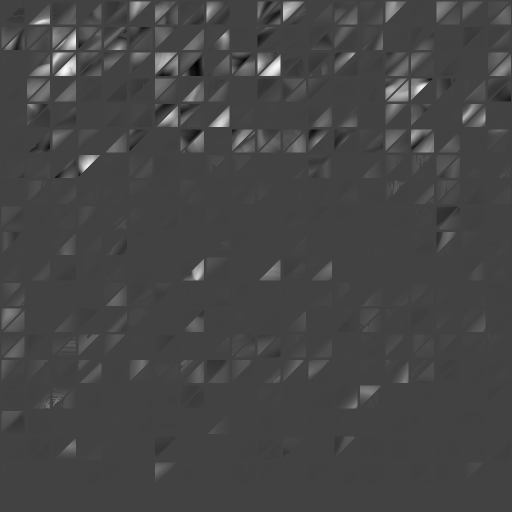
\includegraphics[width=6cm]{../images/dispmap_bunny} \\
{\it (c)} & {\it (d)}
\end{tabular}
\caption[Displacement Maps]{\label{fig:dispmapresults} Displacement Maps. (a) Cubehead. (b) Monster (pelted). (c) Horse. (d) Bunny. See figure \ref{fig:models} for illustration of the associated control and detail layers}.
\end{center}
\end{figure}

We have generated displacement maps for each of the models shown in figure \ref{fig:models}. Texture coordinates for the models were generated in different ways. The Cubehead model, as it only contains 8 vertices, had it's texture coordinates defined by hand. The coordinates for the Monster model were generated using the pelting method described above, in section \ref{sec:dispmapcreation:unwrap}. Pelted maps could not be generated for the Horse and Bunny models however, as the pelting algorithm could not find a bijective mapping for the control meshes, particularly in regions where a number of very small triangles were left over from the detail layer mesh. These models therefore use the regular tiling method of texture coordinate generation.

The resulting displacement maps for each model are shown in figure \ref{fig:dispmapresults}. It is easy to see the shape of the error function for the surface from the images, particularly for the pelted models. The polygonal structure underlying the mesh is also visible in the displacement maps, as darker bands across the image. This is because in most cases, the edges of the control mesh will lie close to the surface.

One problem with automatically decimated control models and regular tiling is illustrated by figures \ref{fig:dispmapresults}c and \ref{fig:dispmapresults}d. These models often contain a number of small triangles that could not be decimated. With regular tiling, these triangles are allocated the same area in the displacement map as large ones that cover much more of the surface area of the model. However,there is much less information to store in these sections, leading to large areas of the resulting displacement map being effectively empty. The pelting method would solve this issue, as such triangles would only occupy a small area in the image, but these examples show that a more effective method of texture coordinate generation needs to be developed to cope with situations in which the pelting fails.

\subsection{\label{sec:dispmapanim:reconstruction:results}Reconstruction Results}

Reconstructions of the displacement maps shown in figure \ref{fig:dispmapresults} can be seen in figure \ref{fig:regen}. Uniform subdivision levels 0, 1, 3, and 5 are shown. As can be seen, the resulting meshes resemble the original surfaces closely.

\begin{figure}
\begin{center}
\begin{tabular}{cccc}
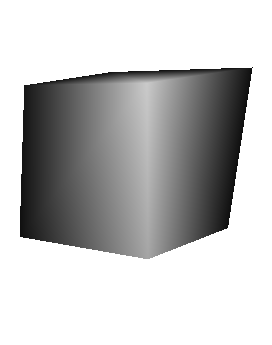
\includegraphics[width=3cm]{../images/cubehead_level0} &
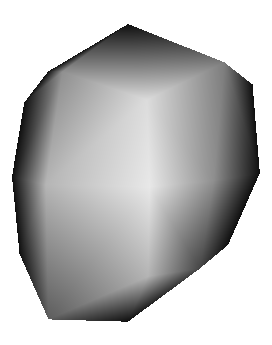
\includegraphics[width=3cm]{../images/cubehead_level1} &
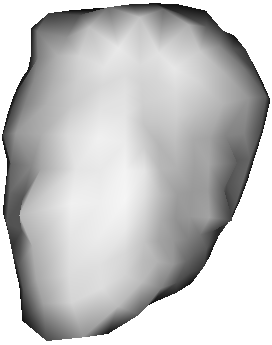
\includegraphics[width=3cm]{../images/cubehead_level3} &
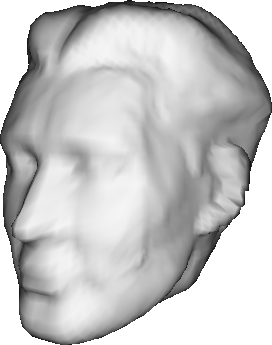
\includegraphics[width=3cm]{../images/cubehead_level5} \\
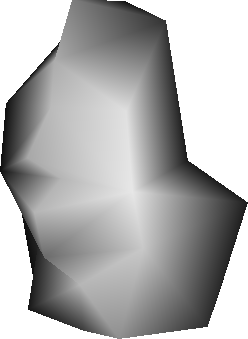
\includegraphics[width=3cm]{../images/dinohead_level0} &
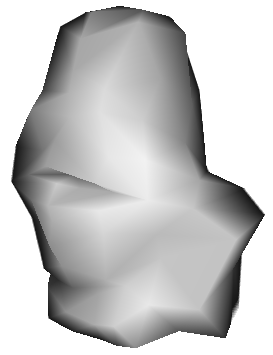
\includegraphics[width=3cm]{../images/dinohead_level1} &
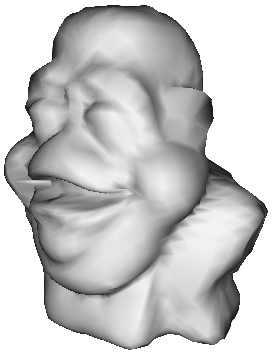
\includegraphics[width=3cm]{../images/dinohead_level3} &
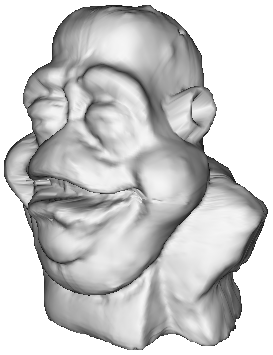
\includegraphics[width=3cm]{../images/dinohead_level5} \\
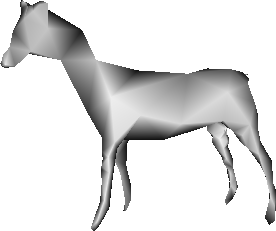
\includegraphics[width=3cm]{../images/horse_level0} &
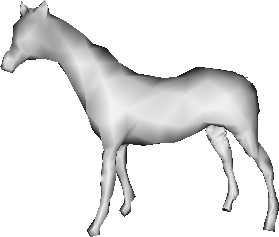
\includegraphics[width=3cm]{../images/horse_level1} &
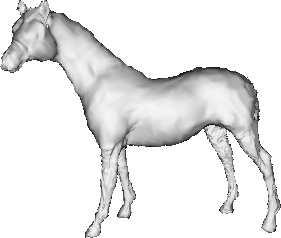
\includegraphics[width=3cm]{../images/horse_level3} &
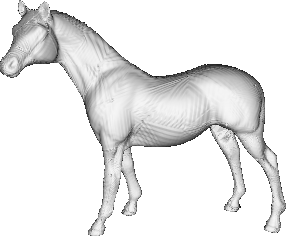
\includegraphics[width=3cm]{../images/horse_level5} \\
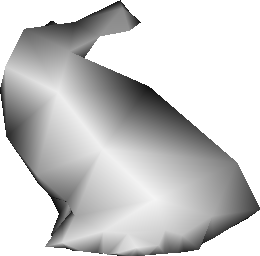
\includegraphics[width=3cm]{../images/bunny_level0} &
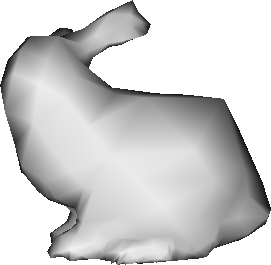
\includegraphics[width=3cm]{../images/bunny_level1} &
\includegraphics[width=3cm]{../images/bunny_level3} &
\includegraphics[width=3cm]{../images/bunny_level5} \\
{\it (a)} & {\it (b)} & {\it (c)} & {\it (d)}
\end{tabular}
\caption[Displacement Map Reconstruction]{\label{fig:regen} Displacement Map Reconstruction. (a) Control layer (b) Level 1 uniform subdivision (c) Level 3 (d) Level 5. }
\end{center}
\end{figure}

\section{\label{sec:dispmapcreation:conclusion}Conclusion}

In this chapter, we have presented a method of representing a dense mesh surface using a displacement map. By building on the layered model approach presented earlier, we can represent a detailed surface using a simplified polygonal control mesh, to which we add a displacement map. The displacement map represents the scalar error function between the control and detail meshes in our original layered model, and allows us to store the mesh in an efficient yet flexible format. We have also presented a complete algorithm for the calculation of this error function based on a mapped detail layer.  This displacement mapped representation can then be rebuilt into a detailed model using a uniform subdivision method. 

Reconstructed displacement mapped meshes closely resemble the original surface data, but in order to justify our method properly, we must analyse the errors introduced by the mapping and reconstruction process. This is dealt with in the next chapter. We will also discuss applications of our displacement maps, as they lend themselves easily to surface compression and editing.
